\subsection{Design of the membrane}
\label{sec: Design_of_the_membrane}
The design goal for the membrane was to create a structure that could support the magnet \textbf{just enough} to win over its gravitational force so that any other force applied to it on the z-axis would be enough to move it and make it vibrate.
For the membrane design, we decided to use a simple Celtic-cross structure as we described previously in section \ref{sec: Membrane-magnet_system}.
This resulted in a membrane with a central cylindrical chamber used to trap the magnet which is \textbf{suspended} by four parallelepipedal arms.
\begin{figure}[H]
    \centering
    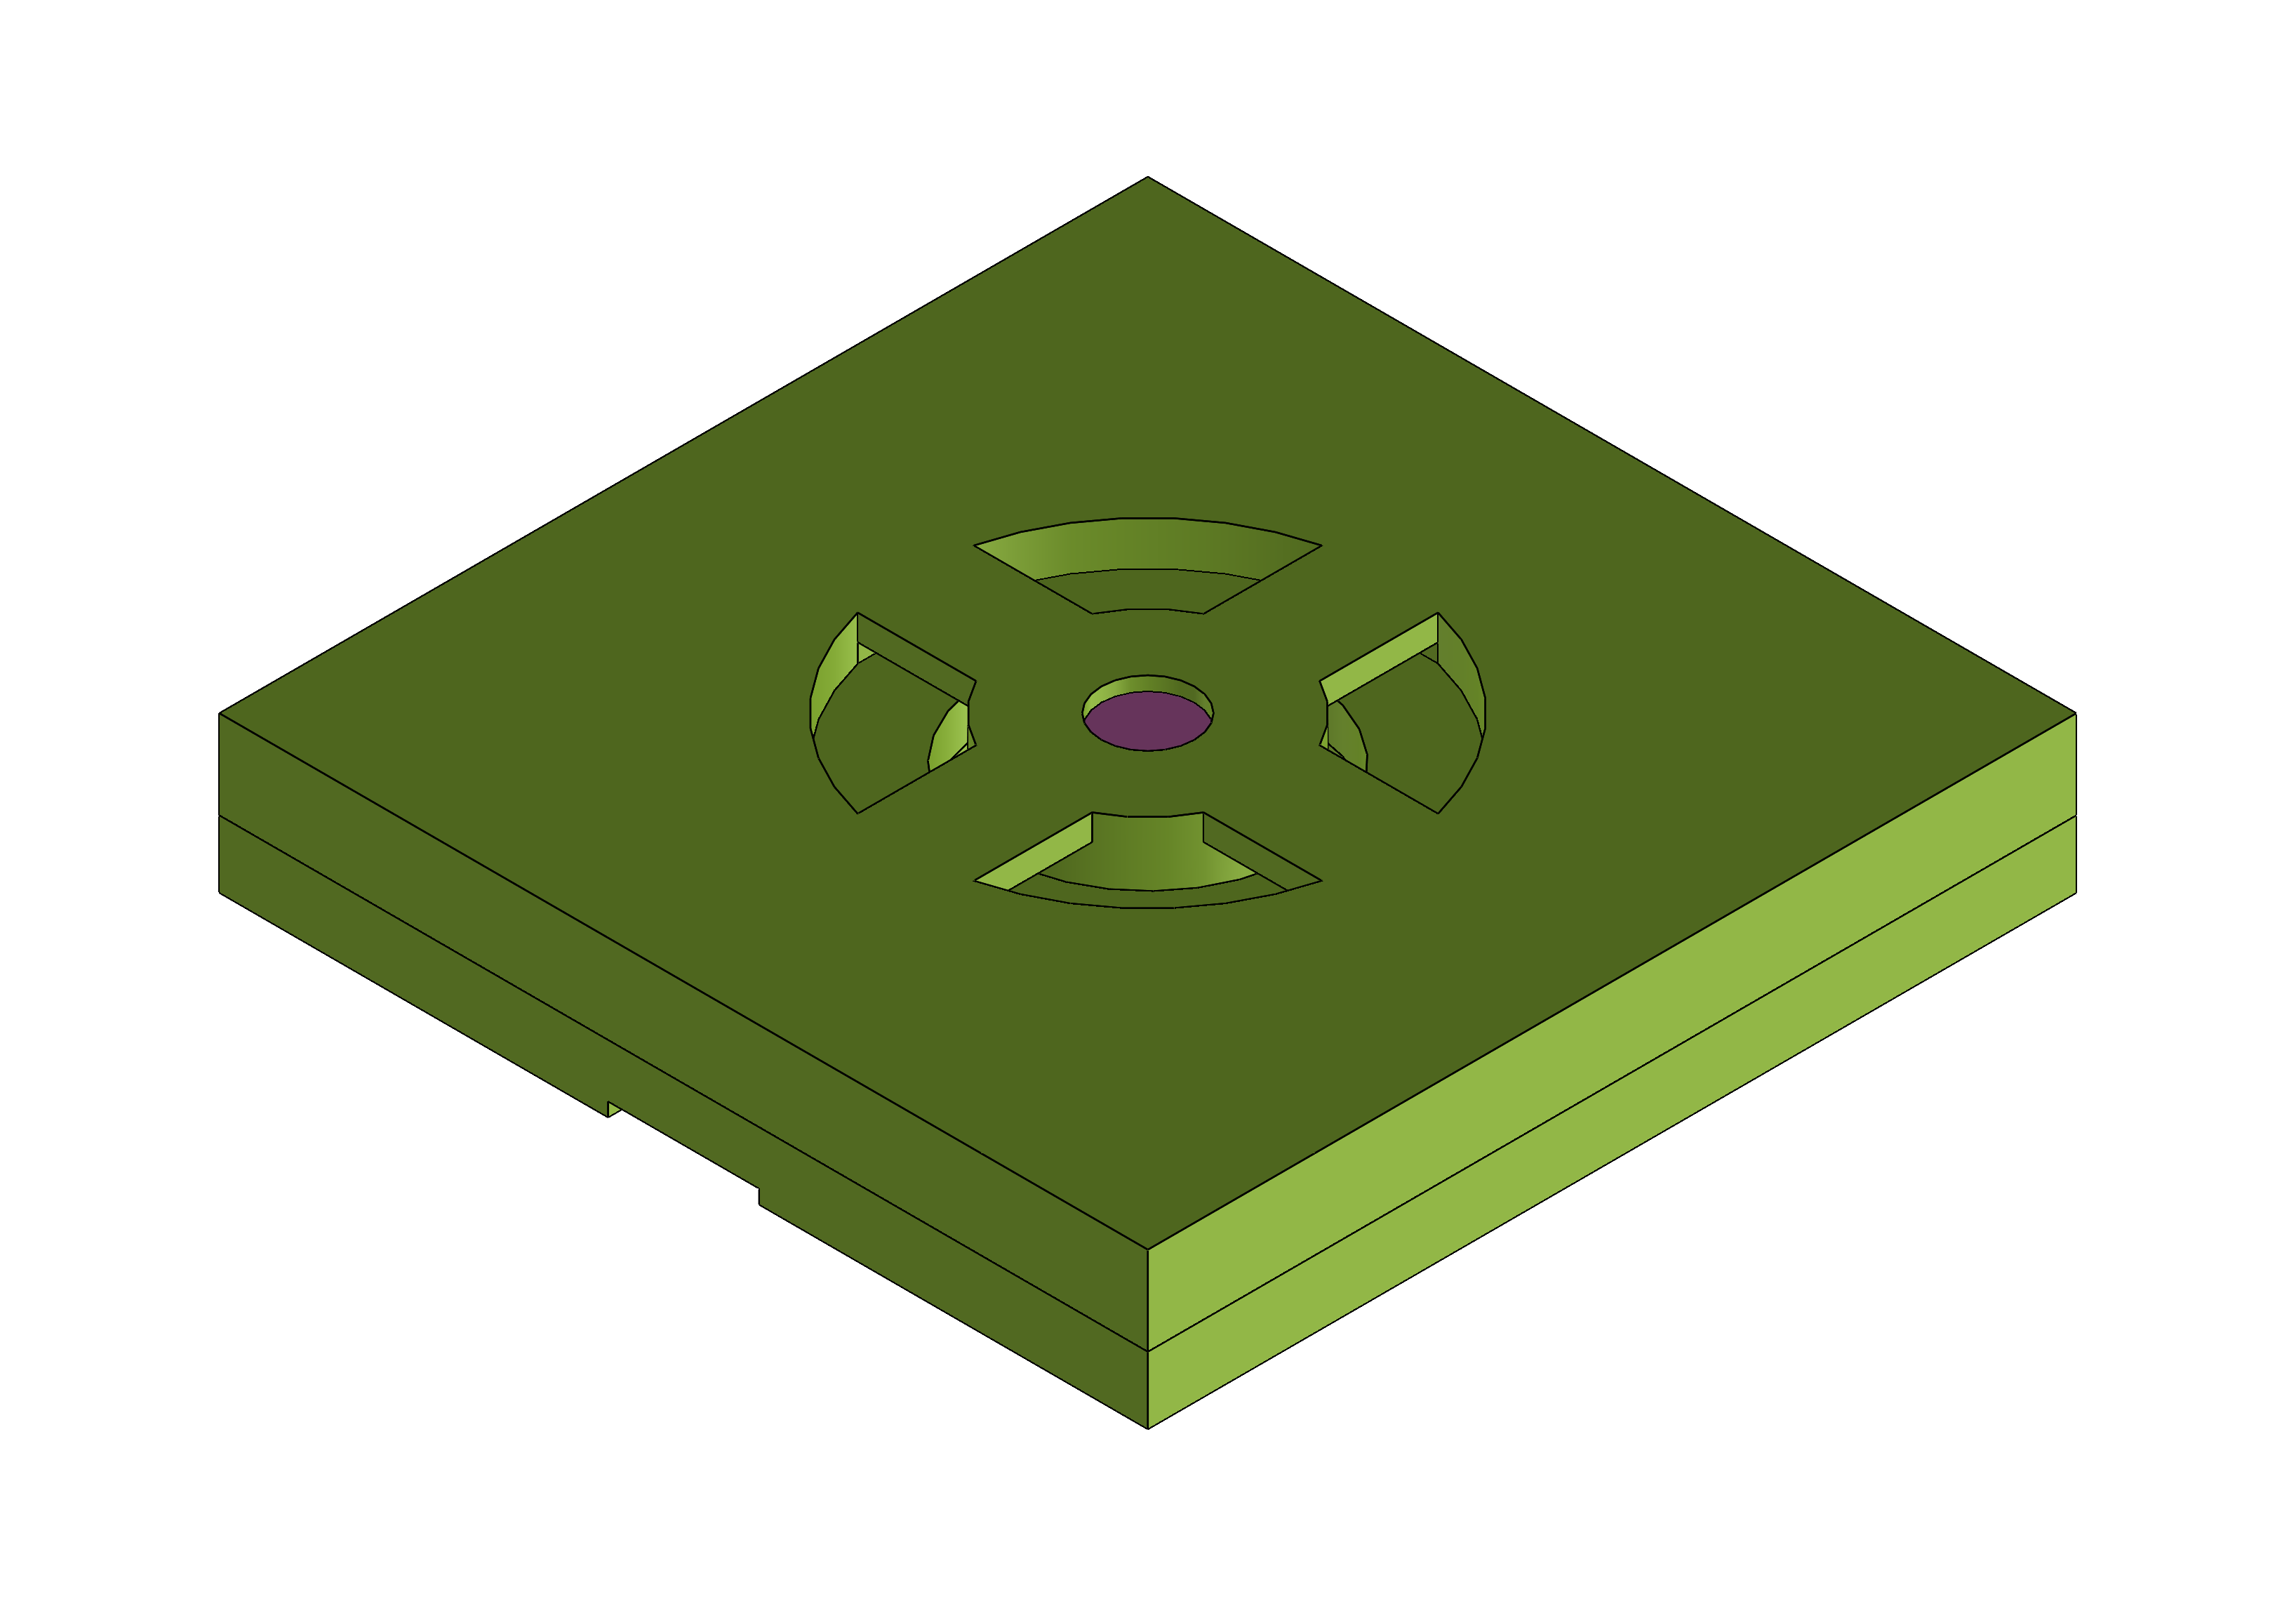
\includegraphics[width=0.7\linewidth]{Chapters/Chapter5/Flexible_Mat_Prototypes/Figures/membrane_v1.png}
    \caption{Membrane top view of the small magnet prototype.}
    \label{fig: Membrane_v1_model}
\end{figure}

\subsubsection{Material stiffness and thickness}
While prototyping we experimented with the same two different silicone materials we described in section \ref{sec: Sleeve_production}.
We quickly realized that the softer silicone was \textbf{too soggy} as the membrane arms would need to be too thick to support the magnet.
We so decided to move forward with only the \textbf{harder silicone} which allowed us to create thinner arms.

\subsubsection{Membrane structure vs magnet dimensions}
The main prototypes we realized were designed with two different N52 cylindrical magnets in mind.
The first one is a small \textbf{10mm} diameter and \textbf{2mm} thick magnet, the second one is a \textbf{15mm} diameter and \textbf{3mm} thick magnet.
The two magnets also have \textbf{very different weights}, the small one weighs \textbf{1.13g} while the big one \textbf{4.03g}.
The first design of the membrane was based on the \textbf{small magnet}, thanks to it being \textbf{lightweight} it could be supported by a membrane with \textbf{very thin arms} (\textbf{0.6mm}) and a width of \textbf{4mm}.
The membrane arms needed also to be \textbf{long enough} to allow the magnet to move freely on the z-axis, so we decided to make them \textbf{4mm} long.
\begin{figure}[H]
    \centering
    \resizebox{0.9\textwidth}{!}{
        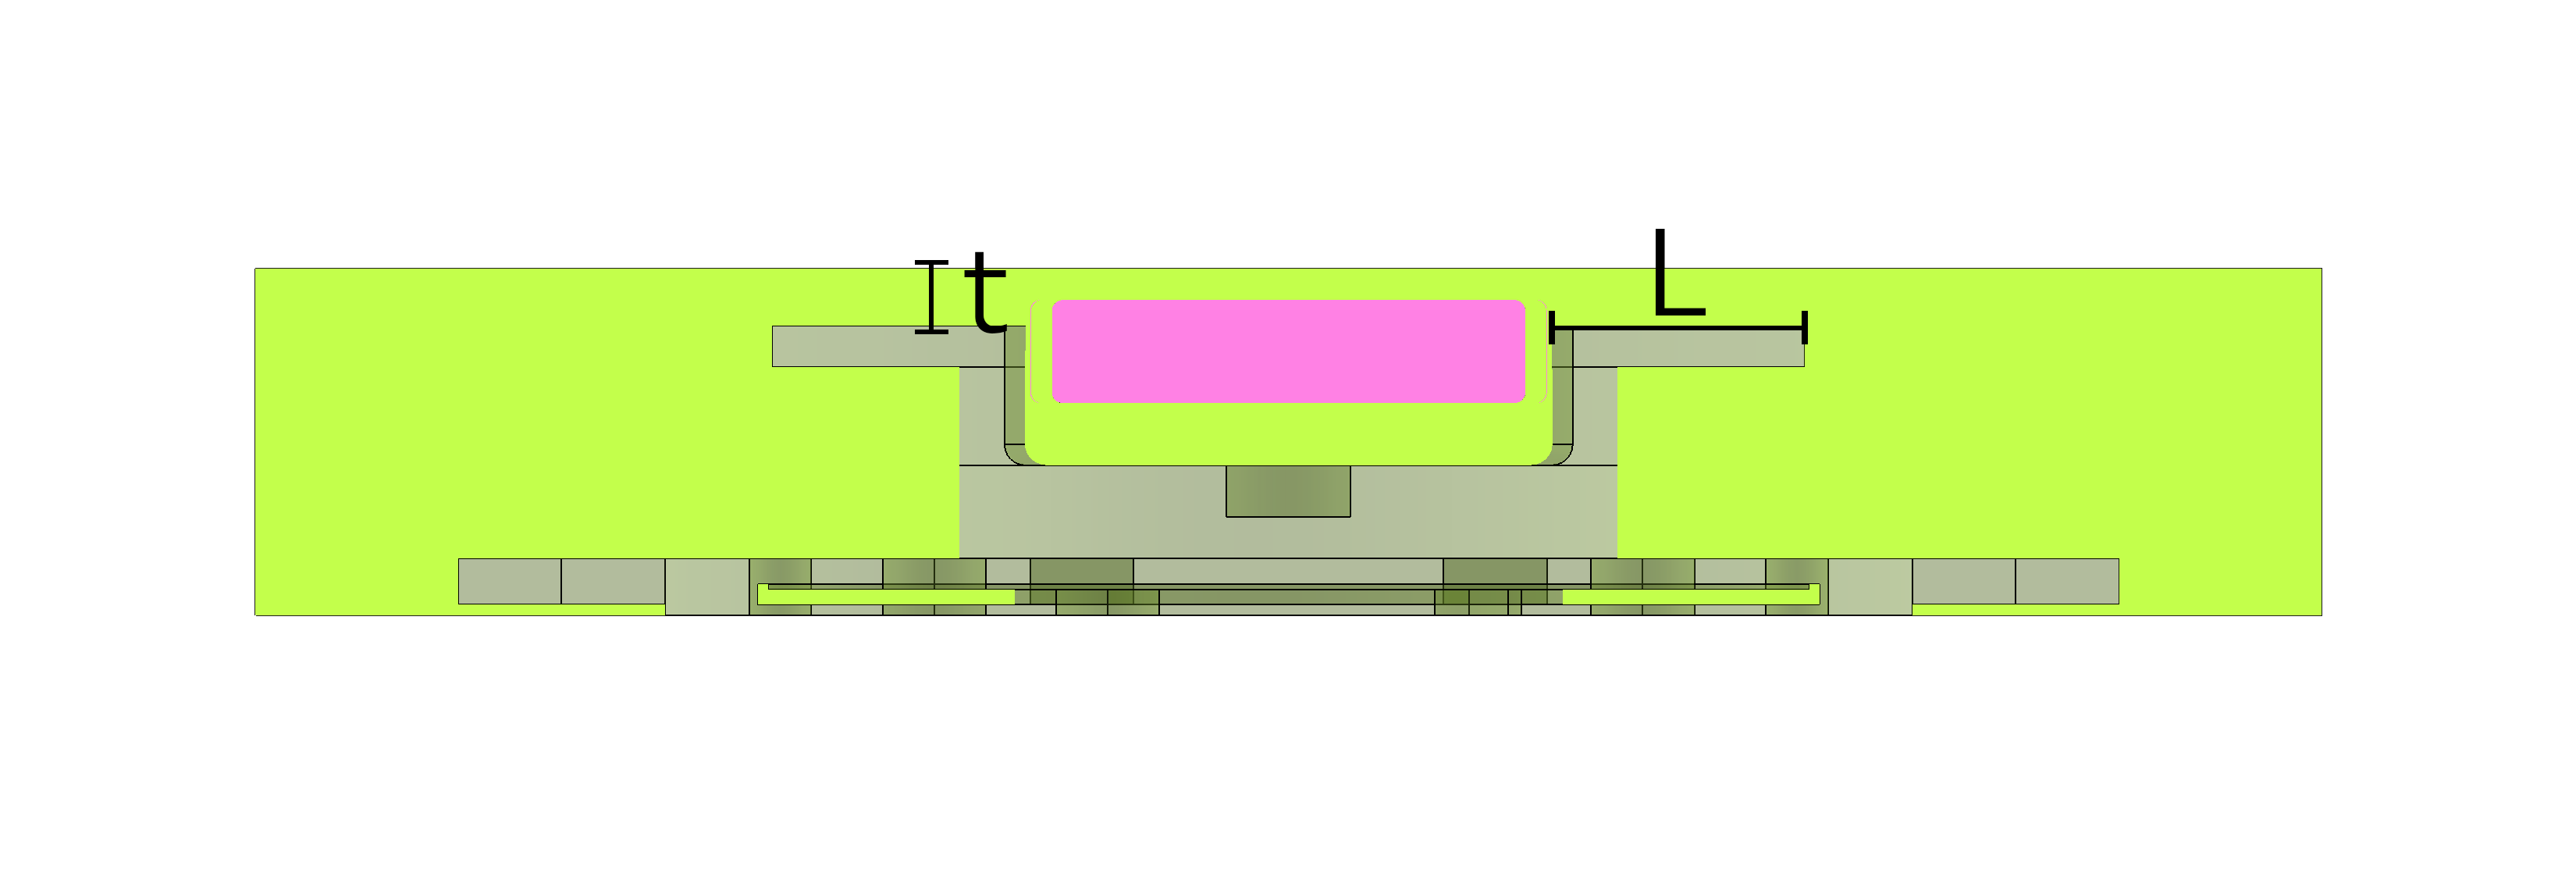
\includegraphics{Chapters/Chapter5/Flexible_Mat_Prototypes/Figures/membrane_v1_section.png}
    }
    \caption{Membrane cross-section of the small magnet prototype (t->thickness, L->length).}
    \label{fig: Membrane_v1_section}
\end{figure}

Switching to the big magnet we realized that the membrane arms would need to be \textbf{thicker} to support the magnet, even if we made them wider (\textbf{5mm}).
This was due to the increased weight of the magnet and the increase in the arms' length (now \textbf{5mm}) we needed to make to allow the magnet to move.
To find the new necessary \textbf{minimal thickness} we used the model described in subsection \ref{sec: Membrane_stiffness}.
We set a \textbf{maximum deflection} of \textbf{0.8mm} for the membrane arms and calculated the thickness needed to support the magnet using equations \ref{eq: Beam_deflection} and \ref{eq: Beam_inertia}.
The results showed that the membrane arms would need to be at least \textbf{1.45mm} thick to support the magnet, so we decided to make them \textbf{1.6mm} thick to have a \textbf{safety margin}.

The next problem we encountered arose when we observed that the membrane arms were \textbf{breaking} at the connection with the cylindrical chamber.
This was due to the \textbf{abrupt change of profile} that was causing a stress concentration at that point.
To solve this problem we decided to add a \textbf{small fillet} to the connection between the arms and the chamber.
\begin{figure}[H]
    \centering
    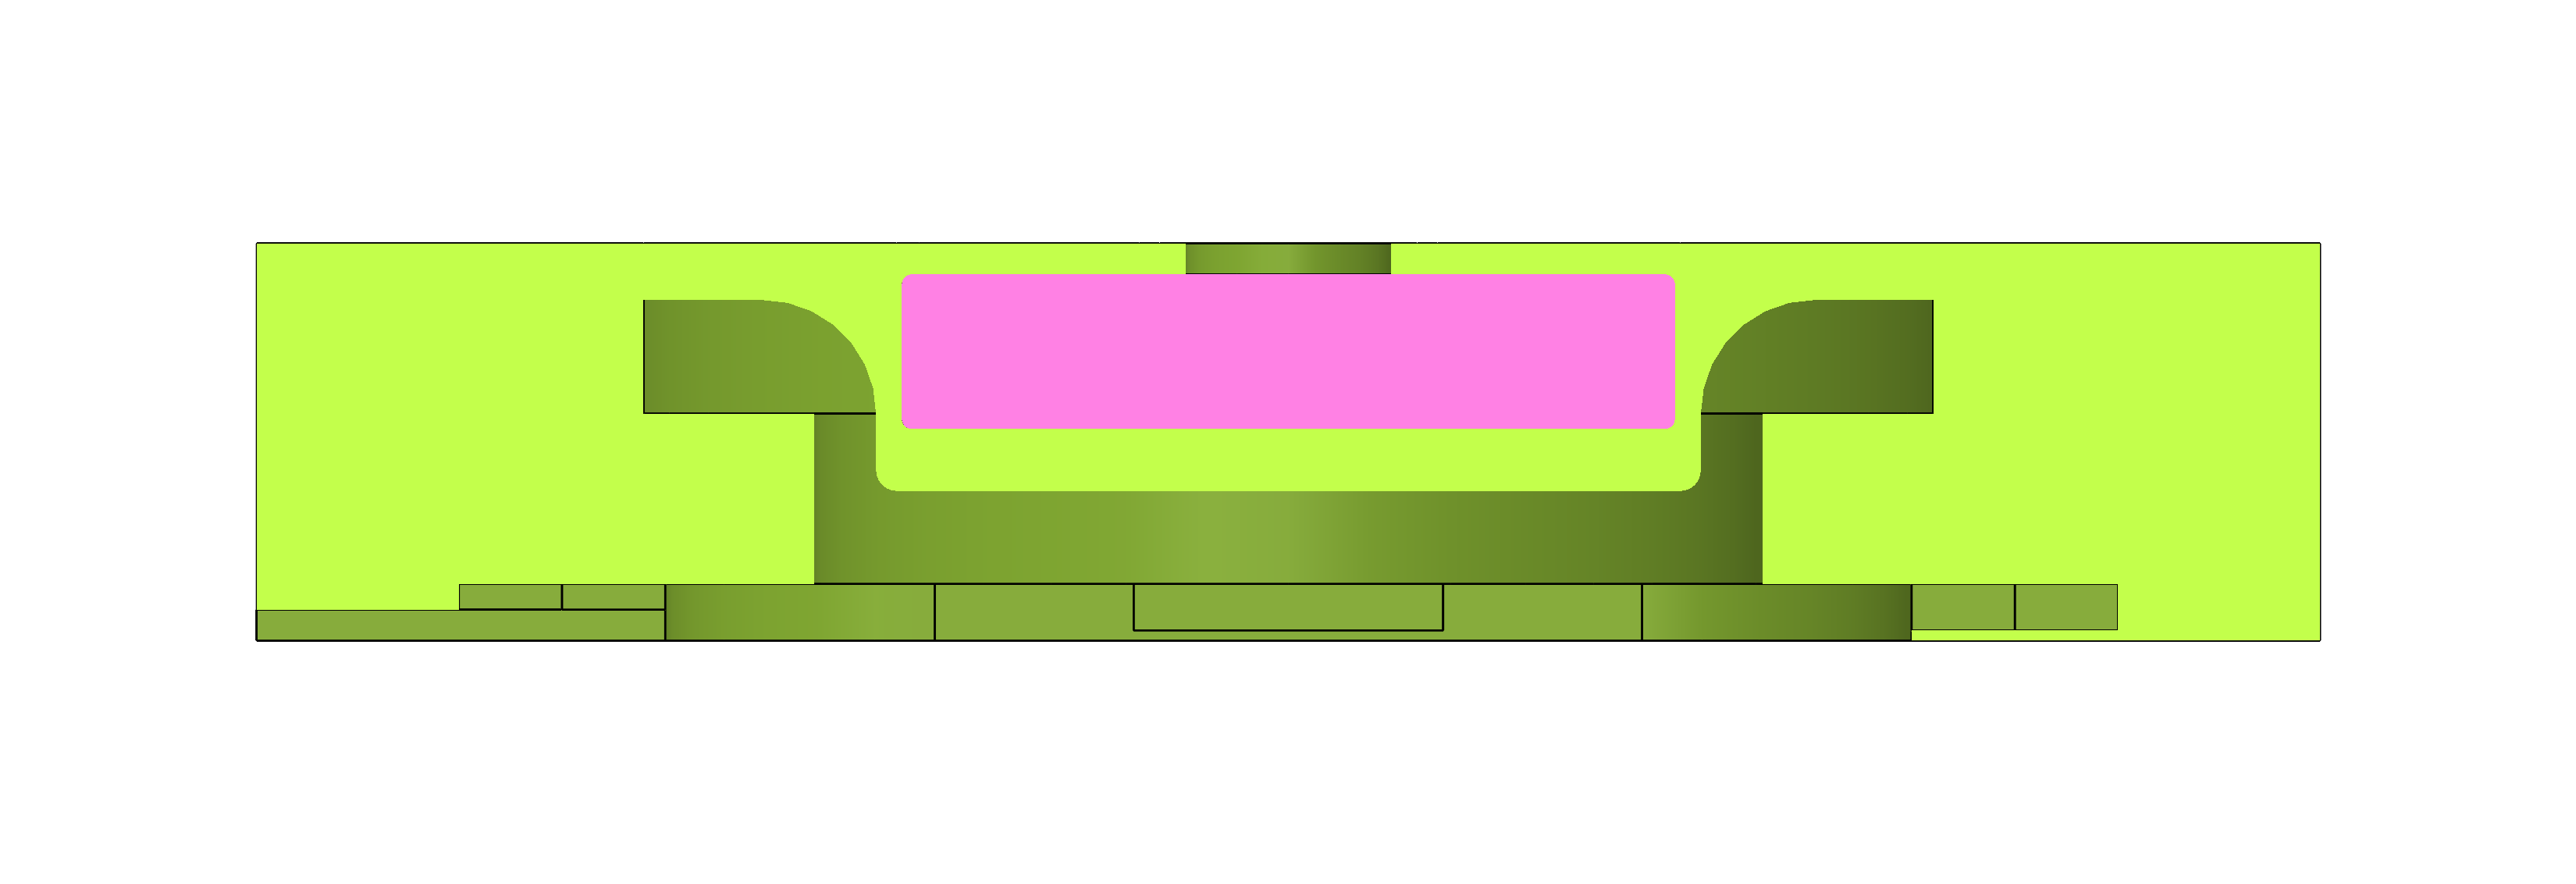
\includegraphics[width=0.9\linewidth]{Chapters/Chapter5/Flexible_Mat_Prototypes/Figures/membrane_v2_section.png}
    \caption{Membrane cross-section of the big magnet prototype.}
    \label{fig: Membrane_v2_section}
\end{figure}